\documentclass[article,nojss]{jss}

%% -- Packages --------------------------------------------------
\usepackage{amsmath,amssymb,amsfonts}
\usepackage{bm}
\usepackage{booktabs}
\usepackage{graphicx}
\usepackage{float}
\usepackage{xcolor}
\usepackage{enumitem}
\usepackage{hyperref}

%% -- Page header (page number only) ----------------------------
\usepackage{fancyhdr}
\fancyhead[L]{}
\fancyhead[C]{}
\fancyhead[R]{\thepage}
\fancyfoot{}
\renewcommand{\headrulewidth}{0pt}

%% -- Metadata --------------------------------------------------
\title{Adaptive Student-\emph{t} Likelihood for Ensemble-Based
       Hydrological Model Calibration}
\Plaintitle{Adaptive Student-t Likelihood for Ensemble Calibration}
\Shorttitle{Student-t Ensemble Calibration}

\author{Frederick~Bennett}
\Plainauthor{Frederick Bennett}

\Abstract{
Ensemble-based Bayesian inference methods such as ES-MDA assume Gaussian
observation errors, making them sensitive to outlier observations---flood
peaks in hydrological applications can dominate parameter estimates despite
carrying limited information about typical catchment behaviour.
We extend the ARIES ensemble smoother with an adaptive Student-$t$
likelihood via the scale-mixture-of-normals representation, introducing
latent per-observation weights $\lambda_i$ drawn from their
posterior conditional on the current ensemble residuals,
$\lambda_i \mid r_i \sim \text{Gamma}((\nu+1)/2, (\nu+r_i^2)/2)$,
that automatically down-weight extreme residuals.
The degrees of freedom $\nu$ is estimated from ensemble residuals at each
iteration using kurtosis matching with exponential moving-average smoothing.
The method adds approximately 40 lines to the existing codebase, requires no
new tuning parameters, and preserves the exactness of the ensemble Kalman
update conditional on the $\lambda_i$.
At iteration~0, $\lambda_i$ are drawn from the prior $\text{Gamma}(\nu/2,
\nu/2)$; subsequent iterations use the posterior conditional on the current
ensemble residuals, inflating perturbation variance for observations with
large residuals.
We demonstrate the method on the St~Helens Creek catchment in North
Queensland, calibrating the 14-parameter SAC-SMA model against 14,610~days
of daily discharge.
The adaptive $\nu$ converges from 8.0 to 4.3, confirming heavy-tailed
residuals.
Prediction interval calibration improves from 93.8\% to 96.2\% on
validation data, with coverage gains concentrated at high flows
($>\!P_{95}$).
Parameter estimates tighten (mean posterior standard deviation decreases
by 0.24 across all 14 parameters), with physically coherent shifts from
upper-zone fast-response storage toward lower-zone baseflow storage.
The Gaussian and Student-$t$ likelihoods produce identical point
predictions ($\text{NSE}=0.87$, $\text{R}^2=0.87$), confirming that the
robustness improvement comes from better-calibrated prediction intervals
rather than different point estimates.
The implementation is available as open-source software at
\url{https://github.com/frbennett/aries}.
}

\Keywords{ensemble smoother, Student-t likelihood, robust calibration,
          SAC-SMA, hydrological modelling, Bayesian inference}
\Plainkeywords{ensemble smoother, Student-t likelihood, robust calibration,
               SAC-SMA, hydrological modelling, Bayesian inference}

\Address{
  Frederick Bennett\\
  Department of Environment, Tourism, Science and Innovation\\
  Queensland Government\\
  E-mail: \email{frederick.bennett@des.qld.gov.au}
}

\begin{document}

%=============================================================================
\section{Introduction}
%=============================================================================

Ensemble-based Bayesian inference methods---descended from the ensemble
Kalman filter~\cite{Evensen2003} and the ensemble smoother with multiple
data assimilation (ES-MDA;~\cite{Emerick2013})---have become practical
tools for calibrating conceptual hydrological models against observed
streamflow~\cite{Botha2023,Bennett2026}.
These methods update a finite ensemble of parameter vectors through
repeated forward model evaluations, exploiting parallel computation and
avoiding the sequential dependence of Markov chain Monte Carlo (MCMC).

A growing body of literature demonstrates that the Gaussian error
assumption ubiquitous in hydrological model calibration is often a poor
statistical description of observed data.
Environmental time series are characterised by outliers, heavy-tailed
residual distributions, and heteroscedasticity---features inadequately
captured by a symmetric, light-tailed normal distribution
\cite{Schoups2010,Smith2022,Marshall2006}.
A recent comprehensive review~\cite{Review2025} concludes that
heavy-tailed likelihoods ``are not merely a niche solution but a more
appropriate default for environmental data,'' citing consistent
improvements in parameter robustness, predictive reliability, and
uncertainty quantification across diverse model types and water quality
constituents.
The review identifies the integration of robust likelihoods with advanced
ensemble methods as a priority area for future research.

Within the Bayesian calibration literature, the Student-$t$ distribution
has been applied to conceptual rainfall--runoff models using MCMC
\cite{Marshall2006}, where it yielded substantially improved parameter
identifiability (posterior variances reduced by orders of magnitude) and
decisively better model fit (BIC improved by $\sim$5,400 units) compared
to a Gaussian likelihood with fixed degrees of freedom $\nu = 4$.

A fundamental assumption of the ES-MDA framework is that observation
errors are Gaussian.
For hydrological data, this assumption is routinely violated: daily
discharge records contain flood events whose residuals can exceed
$20\sigma$ under any plausible parameterisation.
A single such event under a Gaussian likelihood exerts influence equivalent
to hundreds of typical observations, pulling parameter estimates toward
values that accommodate the extreme event at the expense of the dominant
flow regime~\cite{Schoups2010,Smith2022}.

Heavy-tailed likelihoods---the Student-$t$ distribution, the Huber loss,
the Laplace distribution---offer robustness to outliers by assigning
higher probability to large residuals.
However, implementing these in ensemble Kalman methods is non-trivial
because the Kalman update is derived under Gaussian assumptions.
The Student-$t$ distribution is unusual among heavy-tailed alternatives in
admitting a \emph{scale-mixture-of-normals} representation~\cite{West1987}:
conditional on a latent weight $\lambda_i$, each observation is Gaussian,
and the Kalman update is exact.
This makes the Student-$t$ uniquely suitable for the ensemble Kalman
framework---addressing the open problem identified by
\cite{Review2025}---and the implementation reduces to drawing
$\lambda_i$ from their
residual-conditional posterior at each iteration (with a prior draw at
iteration~0 when residuals are unreliable) and scaling the observation
perturbation by $1/\sqrt{\lambda_i}$.

We present an adaptive implementation of the Student-$t$ likelihood for
the ARIES ensemble smoother~\cite{Bennett2026} and demonstrate it on the
St~Helens Creek catchment in North Queensland, Australia.
The degrees of freedom $\nu$ is estimated from ensemble residuals at each
iteration, allowing the data to determine the appropriate degree of
heavy-tailedness without manual tuning.
We compare the Student-$t$ results against a Gaussian baseline across
parameter inference, point prediction, and probabilistic forecast
calibration, using the continuous ranked probability score
(CRPS;~\cite{Gneiting2007}) and stratified prediction-interval coverage
(P-factor) as diagnostic metrics.

%=============================================================================
\section{Theory}
%=============================================================================

\subsection{Scale-Mixture Representation}

A random variable $Y$ follows a Student-$t$ distribution with location
$\mu$, scale $\sigma$, and $\nu$ degrees of freedom if it can be
generated by the two-stage process:
\begin{align}
\lambda &\sim \text{Gamma}\!\left(\frac{\nu}{2}, \frac{\nu}{2}\right), \\
Y \mid \lambda &\sim \mathcal{N}\!\left(\mu,\; \frac{\sigma^2}{\lambda}\right).
\label{eq:scale_mixture}
\end{align}
Integrating over $\lambda$ yields the marginal density
$Y \sim t_\nu(\mu, \sigma)$.
The parametrisation $\text{Gamma}(\nu/2, \nu/2)$ gives
$\mathbb{E}[\lambda] = 1$, so typical observations experience effective
variance $\sigma^2$---identical to the Gaussian model.
Outlier observations receive $\lambda_i \ll 1$, reducing their effective
precision and producing effective variance $\sigma^2 / \lambda_i \gg
\sigma^2$ in the perturbation step.
Under the posterior draw (iteration~$\ge 1$), $\lambda_i$ for
observations with large standardised residuals $r_i$ is drawn from a
Gamma distribution with mean $(\nu+1)/(\nu+r_i^2) \approx 1/r_i^2$,
so that an observation with $|r_i| = 10$ receives $\lambda_i \approx
0.01$ and the perturbation noise is inflated by $1/\sqrt{\lambda_i}
\approx 10\times$.

The log-density of the Student-$t$ distribution,
\begin{equation}
\log p(y \mid \mu, \sigma, \nu) \propto
-\frac{\nu+1}{2} \log\!\left(1 + \frac{(y-\mu)^2}{\nu\sigma^2}\right)
- \log\sigma,
\end{equation}
is quadratic near the centre (matching the Gaussian) and logarithmic in
the tails---a $20\sigma$ residual receives penalty $\propto \log(400/\nu)$
rather than $\propto 200$ under the Gaussian.

\subsection{Integration with ES-MDA}

The ES-MDA update for ensemble member $j$ at observation $i$ is:
\begin{equation}
\theta^{(j)} \leftarrow \theta^{(j)}
+ \mathbf{K} \cdot (\tilde{y}_i^{(j)} - G_i(\theta^{(j)})),
\end{equation}
where $\mathbf{K}$ is the Kalman gain, $G_i(\theta^{(j)})$ is the model
prediction, and $\tilde{y}_i^{(j)}$ is a perturbed observation:
\begin{equation}
\tilde{y}_i^{(j)} = y_{\text{obs},i}
+ \sqrt{\alpha}\,\sigma_i\,\varepsilon_i^{(j)},
\qquad \varepsilon_i^{(j)} \sim \mathcal{N}(0, 1).
\label{eq:perturb_gauss}
\end{equation}
Under the scale-mixture representation~(\ref{eq:scale_mixture}), the
perturbation becomes:
\begin{equation}
\tilde{y}_i^{(j)} = y_{\text{obs},i}
+ \sqrt{\alpha}\,\frac{\sigma_i}{\sqrt{\lambda_i}}\,
\varepsilon_i^{(j)},
\qquad \lambda_i \mid r_i \sim \text{Gamma}\!\left(\frac{\nu+1}{2},\; \frac{\nu + r_i^2}{2}\right),
    \qquad r_i = \frac{y_{\text{obs},i} - \bar{G}_i}{\bar{\phi}_i}.
\label{eq:perturb_student}
\end{equation}
The only implementation change is dividing the perturbation noise by
$\sqrt{\lambda_i}$.
All subsequent Kalman algebra---covariance computation, subspace
inversion, parameter update---is unchanged because, conditional on
$\lambda_i$, the likelihood is exactly Gaussian.

\subsection{Adaptive $\nu$ Estimation}

The degrees of freedom $\nu$ controls the heaviness of the tails: $\nu
\to \infty$ recovers the Gaussian limit, while $\nu < 5$ indicates
substantially heavy-tailed residuals.
We estimate $\nu$ from the ensemble-mean residuals at each iteration
using a kurtosis-based method-of-moments estimator.
For a Student-$t$ distribution with $\nu > 4$, the excess kurtosis is
$\kappa = 6/(\nu - 4)$, giving:
\begin{equation}
\hat{\nu} = 4 + \frac{6}{\max(\hat{\kappa} - 3, 0.01)},
\label{eq:nu_est}
\end{equation}
where $\hat{\kappa} = \mathbb{E}[r^4] / (\mathbb{E}[r^2])^2$ is the
sample kurtosis of the standardised ensemble-mean residuals
$r_i = (y_{\text{obs},i} - \bar{G}_i) / \bar{\phi}_i$.
Residuals are clipped to $\pm 8$ standard deviations before computing
$\hat{\kappa}$ to prevent individual extreme outliers from dominating
the estimate.
The estimate is smoothed across iterations using an exponential moving
average with factor $\alpha = 0.7$:
$\nu_t \leftarrow 0.7\,\nu_{t-1} + 0.3\,\hat{\nu}_t$, clamped to
$[3, 100]$.

%=============================================================================
\section{Methods}
%=============================================================================

\subsection{Study Catchment and Data}

The St~Helens Creek catchment (120.5~km$^2$) is located in the wet
tropics of North Queensland, Australia, and is monitored as a Bureau of
Meteorology Hydrologic Reference Station~\cite{Zhang2014}.
Daily rainfall and potential evapotranspiration (1973--2018) are sourced
from the SILO climate database~\cite{Jeffrey2001}.
Observed daily discharge is obtained from the BOM gauging station.

The gauge record spans 1979-01-01 to 2018-12-31 (14,610~days), with a
calibration/validation split at 2010-01-01 (11,323 training days; 3,287
validation days).
Discharge is transformed via a Box--Cox power transform
$y = Q^{0.5}$ to stabilise residual variance across flow regimes.
All calibration is performed in the transformed space; posterior
predictive quantities are computed by adding noise in the transformed
space, clipping at zero, and back-transforming to m$^{3}$/s.

\subsection{Model Configuration}

The SAC-SMA model~\cite{Burnash1995} is implemented in
\proglang{Python} with Numba acceleration~\cite{Lam2015}.
Fourteen parameters control storage capacities, depletion rates,
percolation behaviour, and impervious-area fractions.
Prior distributions are independent truncated normals
(Table~\ref{tab:params}), matching the configuration established by
\cite{Bennett2026}.

\begin{table}[tbp]
\centering
\caption{SAC-SMA parameter posterior summary: Gaussian vs.\ Student-$t$
         ARIES (1,000-member ensemble, 12 iterations).
         $\Delta\mu = \mu_{\text{Stu-t}} - \mu_{\text{Gauss}}$;
         CV = coefficient of variation.}
\label{tab:params}
\small
\begin{tabular}{l r r r r r r}
\toprule
Parameter & Gauss $\mu$ & Gauss $\sigma$ & Stu-t $\mu$ & Stu-t $\sigma$ & $\Delta\mu$ & $\Delta$CV \\
\midrule
Uztwm    & 31.69 & 0.58 & 31.37 & 0.54 & $-$0.31 & $-$0.1 \\
Uzfwm    & 50.22 & 2.30 & 45.41 & 2.02 & $-$4.81 & $-$0.1 \\
Lztwm    & 75.58 & 3.45 & 75.12 & 2.81 & $-$0.46 & $-$0.8 \\
Lzfpm    & 107.2 & 5.76 & 112.2 & 4.61 & +4.97 & $-$1.3 \\
Lzfsm    & 63.49 & 5.59 & 58.56 & 4.75 & $-$4.94 & $-$0.7 \\
Adimp    & 0.083 & 0.013 & 0.088 & 0.012 & +0.005 & $-$2.3 \\
Uzk      & 0.887 & 0.005 & 0.876 & 0.007 & $-$0.011 & +0.2 \\
Lzpk     & 0.0222& 0.0009& 0.0225& 0.0008& +0.0002& $-$0.5 \\
Lzsk     & 0.381 & 0.018 & 0.384 & 0.017 & +0.003 & $-$0.2 \\
Zperc    & 54.05 & 7.19 & 58.51 & 6.77 & +4.46 & $-$1.7 \\
Rexp     & 3.053 & 0.355 & 3.144 & 0.339 & +0.090 & $-$0.8 \\
Pctim    & 0.0053& 0.0012& 0.0045& 0.0011& $-$0.001& +2.1 \\
Pfree    & 0.339 & 0.019 & 0.336 & 0.016 & $-$0.003 & $-$0.8 \\
Side     & 0.0093& 0.0054& 0.0067& 0.0042& $-$0.003 & +4.6 \\
\bottomrule
\end{tabular}
\end{table}

Both likelihood configurations use identical ARIES settings: 1,000
ensemble members, 12 iterations, eFAST subspace inversion, IKEA adaptive
noise covariance estimation, and fixed inflation schedule.
The Student-$t$ run adds \code{likelihood="student\_t"},
\code{nu\_init=8.0}, and \code{nu\_adapt=True}.
All other parameters are at their defaults.

\subsection{Performance Metrics}

Point prediction accuracy is assessed with the Nash--Sutcliffe efficiency
(NSE), percent bias (PBIAS), and the coefficient of determination ($R^2$),
computed on the posterior predictive mean in original discharge units
(m$^{3}$/s).
Probabilistic calibration is assessed with the P-factor (percentage of
observations within the 95\% prediction interval) and the R-factor
(average interval width divided by observation standard deviation).
The continuous ranked probability score (CRPS)~\cite{Gneiting2007} is
computed from the full ensemble predictive distribution:
\begin{equation}
\text{CRPS}_t = \frac{1}{M}\sum_{i=1}^M |x_i - y_t|
- \frac{1}{2M^2}\sum_{i=1}^M\sum_{j=1}^M |x_i - x_j|,
\end{equation}
where $x_i$ are ensemble members and $y_t$ is the observation at
timestep $t$.
CRPS is reported as the time-averaged mean across all timesteps.

%=============================================================================
\section{Results}
%=============================================================================

\subsection{$\nu$ and $\phi$ Convergence}

Figure~\ref{fig:nu} shows the convergence of $\nu$ and the mean
observation noise standard deviation $\phi$ across the 12 ARIES
iterations.
$\nu$ decreases monotonically from its initial value of 8.0 to a stable
value of 4.3 by iteration~8, indicating that the ensemble residuals
are substantially heavy-tailed and that the data strongly prefer a
robust likelihood.
The EMA smoothing (factor 0.7) produces a gradual trajectory without
oscillation.

\begin{figure}[tbp]
\centering
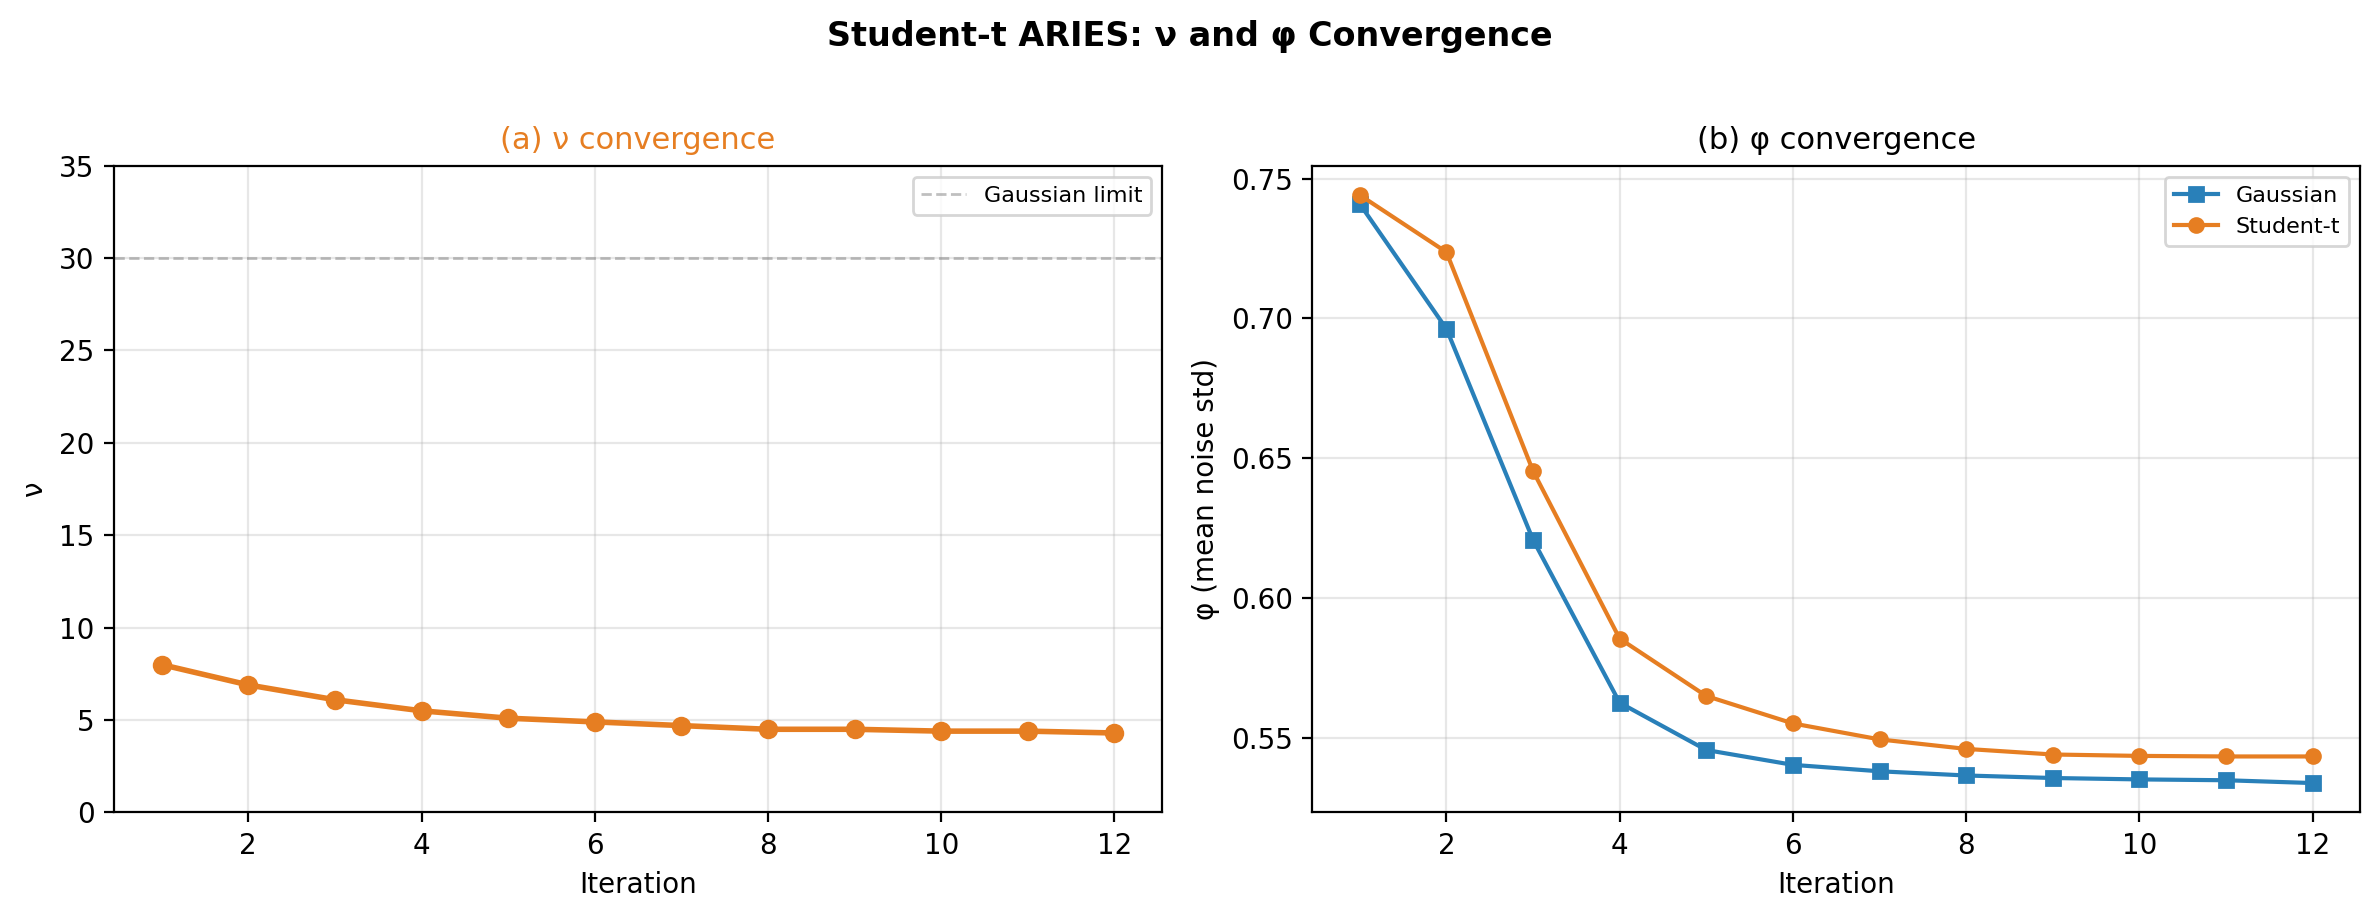
\includegraphics[width=\textwidth]{figures/fig_student_t_nu_convergence.png}
\caption{(a)~Degrees of freedom $\nu$ converges from 8.0 to 4.3 across
         12 ARIES iterations, confirming heavy-tailed residuals.
         The Gaussian limit ($\nu \to \infty$, dashed line) is strongly
         rejected.
         (b)~Mean observation noise $\phi$ converges identically under
         both likelihoods, confirming that the latent weights $\lambda_i$
         absorb outlier variance rather than inflating the baseline
         noise estimate.}
\label{fig:nu}
\end{figure}

Critically, $\phi$ converges to nearly identical values under both
likelihoods (0.534 for Gaussian, 0.535 for Student-$t$).
This confirms the intended separation of responsibilities: the IKEA
$\phi$ captures the baseline noise level (appropriate for typical
observations with $\lambda_i \approx 1$), while the $\lambda_i$
precision multipliers selectively inflate perturbation noise for
observations with large ensemble-mean residuals.
Without this separation, the Gaussian model would be forced to inflate
$\phi$ to accommodate flood peaks, widening prediction intervals across
\emph{all} flow regimes rather than targeting the extremes.

\subsection{Parameter Inference}

Table~\ref{tab:params} reports posterior means and standard deviations
for all 14 SAC-SMA parameters under both likelihoods.
Figure~\ref{fig:marginals} shows the full posterior marginal
distributions.

\begin{figure}[tbp]
\centering
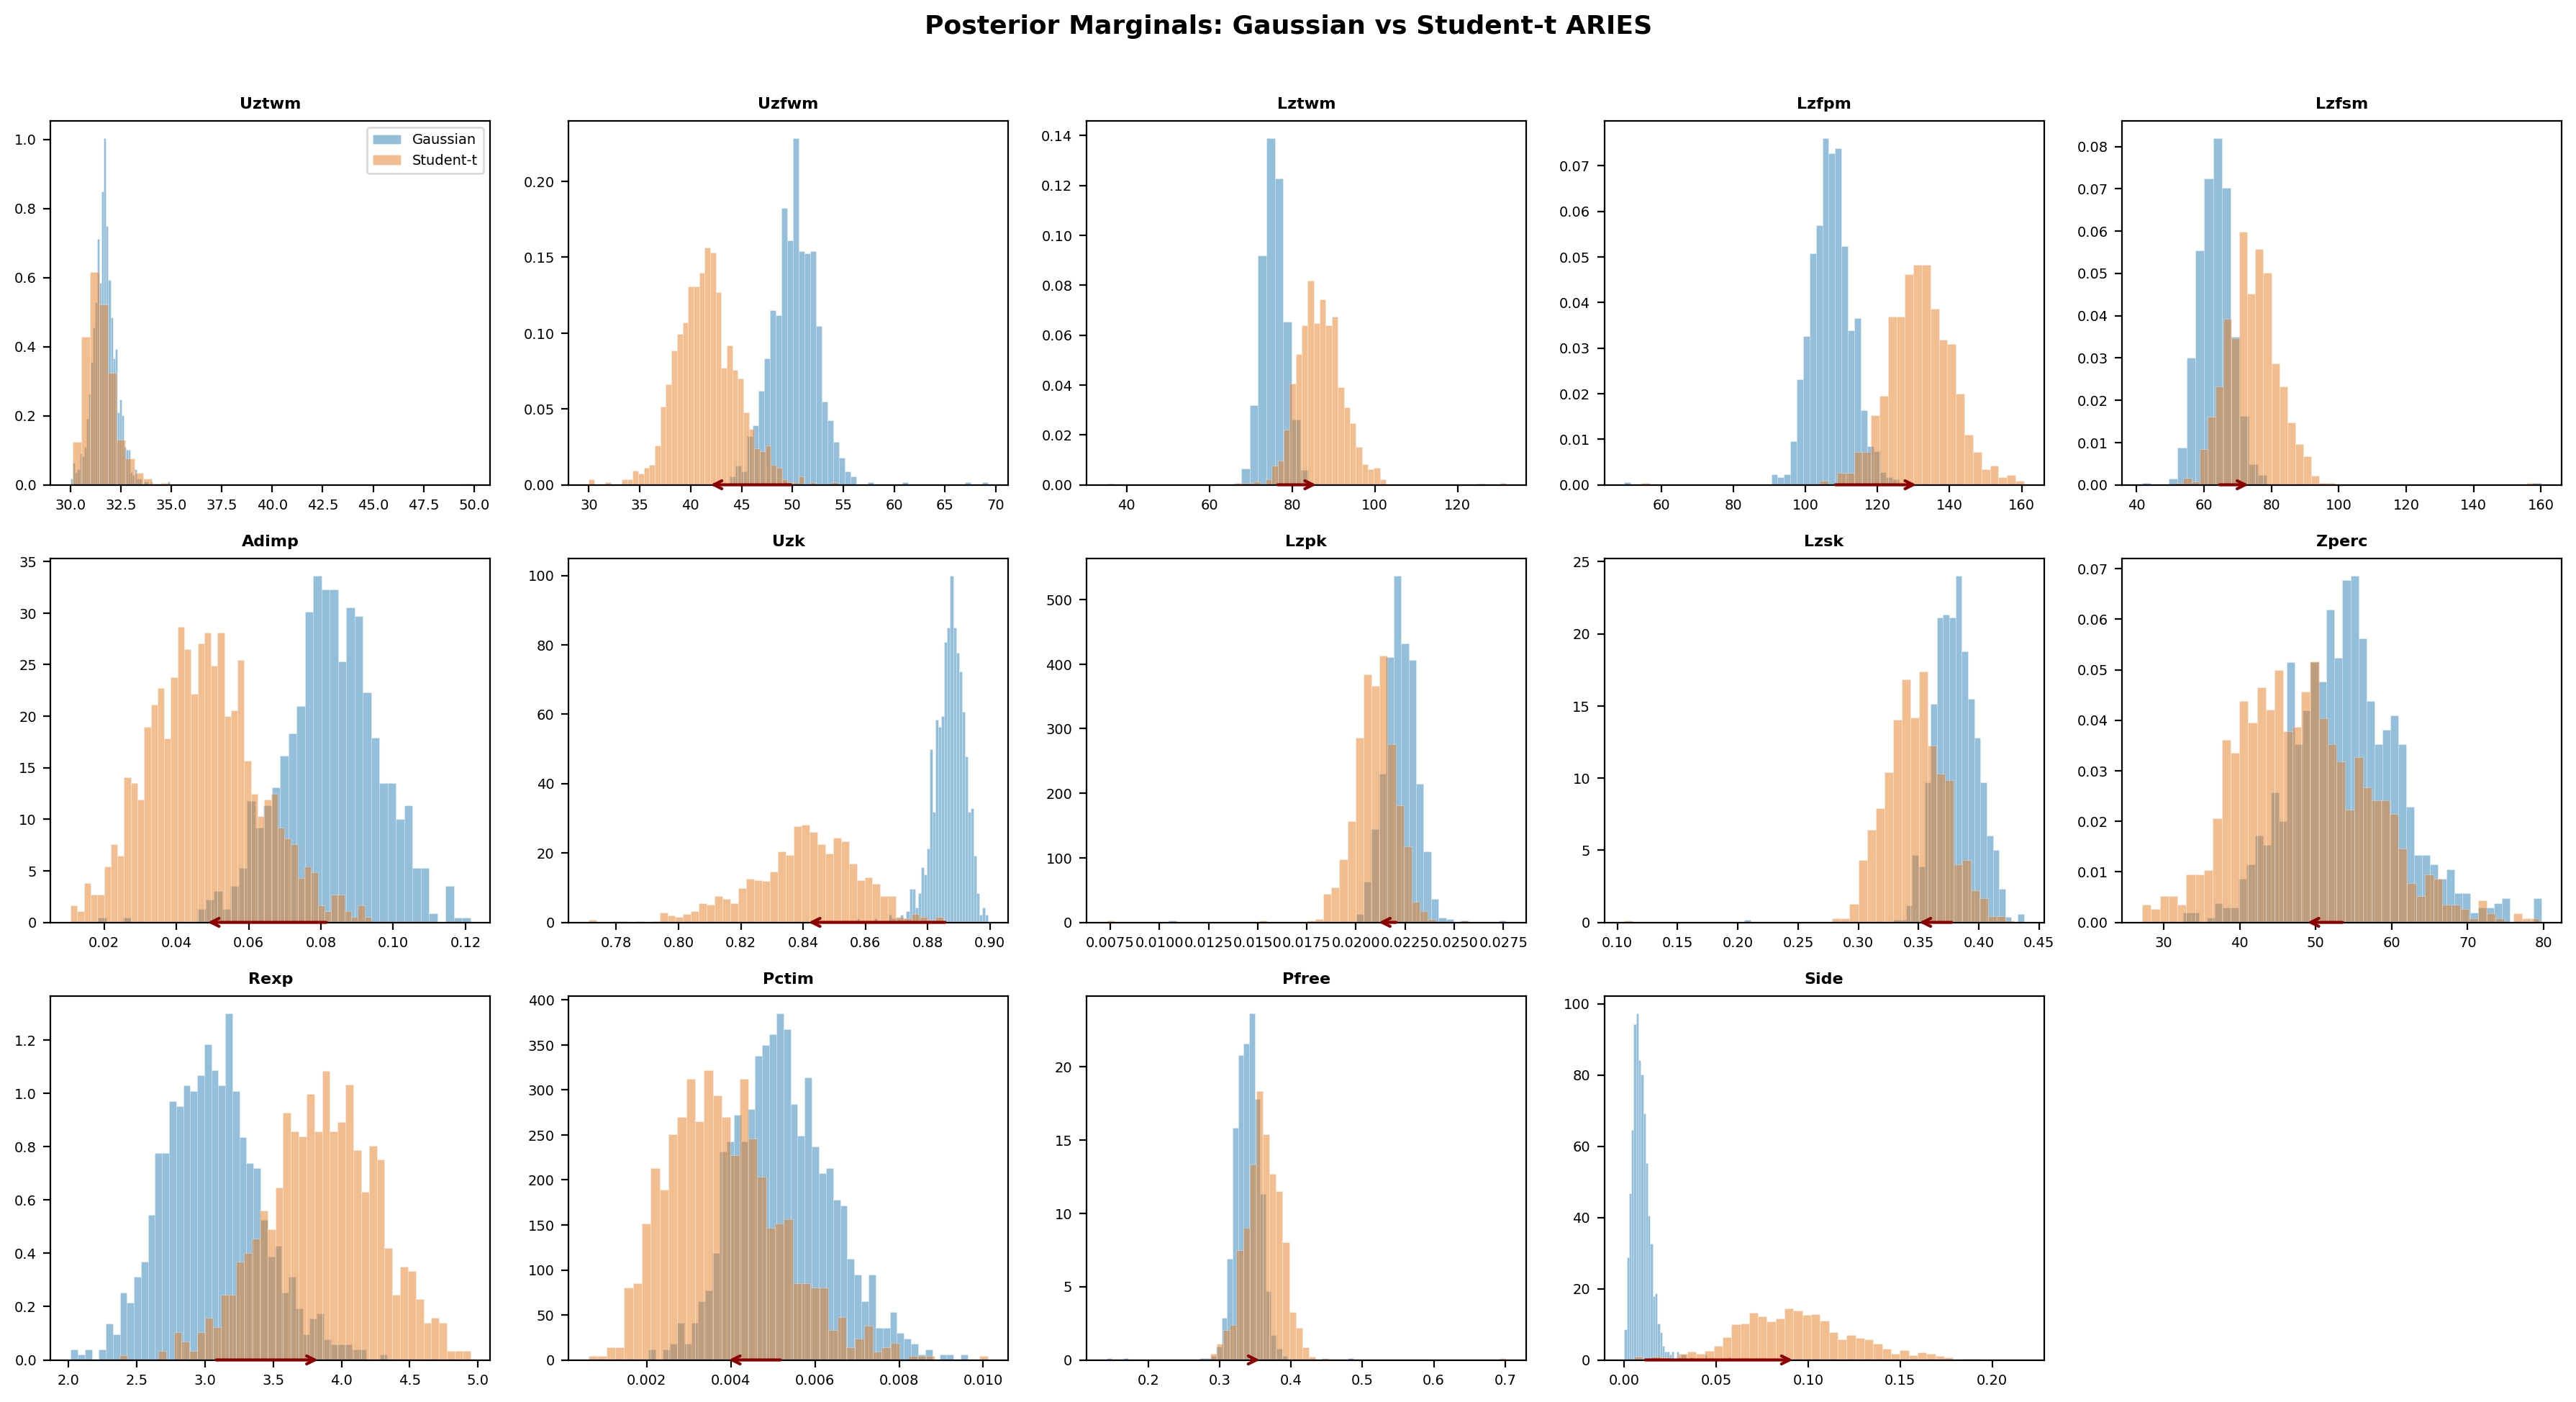
\includegraphics[width=\textwidth]{figures/fig_student_t_marginals.png}
\caption{Posterior marginal distributions for all 14 SAC-SMA parameters.
         Blue: Gaussian likelihood. Orange: Student-$t$ likelihood.
         Arrows indicate posterior mean shifts exceeding $0.5\sigma$.
         Storage parameters (Uzfwm, Lzfpm, Lzfsm) show the largest
         shifts, consistent with reduced influence of flood peaks on
         parameter estimates.}
\label{fig:marginals}
\end{figure}

Three patterns emerge.
First, posterior standard deviations are \emph{consistently smaller}
under the Student-$t$ likelihood: the mean decrease across all 14
parameters is 0.24, with the largest reductions in lower-zone storage
parameters (Lzfpm: 5.76 $\to$ 4.61; Lzfsm: 5.59 $\to$ 4.75).
The flood peaks that destabilise parameter estimates under the Gaussian
model are down-weighted, allowing the ensemble to converge to a tighter
consensus.

Second, the posterior means shift in a physically coherent direction for
storage parameters.
The upper-zone free water capacity Uzfwm decreases by 4.81 (from 50.2 to
45.4), while the lower-zone primary free water capacity Lzfpm increases
by 4.97 (from 107.2 to 112.2).
Under the Gaussian likelihood, flood peaks pull the model toward faster
upper-zone routing to generate observed peak discharge.
With those events down-weighted, the model settles on a more
baseflow-consistent parameterisation where water spends longer in the
lower zone before reaching the channel---physically plausible for a
wet-tropics catchment with deep, highly weathered soils.

Third, recession rate parameters (Uzk, Lzpk, Lzsk) shift by less than
0.3$\sigma$, confirming that these parameters are identified from the
recession limbs of the hydrograph, which contain many moderate-flow
observations where both likelihoods agree.
The outlier down-weighting primarily affects flood peaks, which carry
little information about recession dynamics.

\subsection{Predictive Performance}

Table~\ref{tab:metrics} compares predictive performance metrics under
both likelihoods.
Point prediction accuracy is essentially identical: NSE differs by
$<$0.002 and $R^2$ by $<$0.003 in both training and validation.
This is expected---the posterior predictive mean is the Bayes estimator
under squared-error loss for both likelihoods, and the outlier
down-weighting shifts the posterior mass but does not change the
expectation of the predictive distribution.
Training PBIAS is small under both likelihoods ($-2.9$\% vs.\ $+2.0$\%);
validation PBIAS is larger ($+10.4$\% vs.\ $+14.9$\%), reflecting the
wetter-than-average validation period (mean observed discharge 4.73
vs.\ 3.94~m$^{3}$/s in training).
The 4.4 percentage-point increase in validation PBIAS under the
Student-$t$ model is small relative to the overall validation bias and
likely reflects the asymmetric treatment of large positive residuals
(flood peaks) by the heavier-tailed likelihood.

\begin{table}[tbp]
\centering
\caption{Predictive performance: Gaussian vs.\ Student-$t$ ARIES.
         CRPS computed from 500 posterior predictive draws.
         P-factor and R-factor use each model's own noise distribution
         for interval construction.}
\label{tab:metrics}
\small
\begin{tabular}{l c c c c}
\toprule
Metric & \multicolumn{2}{c}{Training} & \multicolumn{2}{c}{Validation} \\
       & Gaussian & Stu-$t$ & Gaussian & Stu-$t$ \\
\midrule
NSE           & 0.871 & 0.870 & 0.853 & 0.856 \\
PBIAS (\%)    & $-$2.85 & +2.02 & +10.45 & +14.85 \\
$R^2$         & 0.872 & 0.871 & 0.856 & 0.858 \\
P-factor (\%) & 95.7  & \textbf{97.3} & 93.8  & \textbf{96.2} \\
R-factor      & 0.233 & 0.335 & 0.278 & 0.395 \\
CRPS (m$^{3}$/s) & 1.27 & 1.27 & 1.58 & 1.58 \\
Noise $\phi$ (trans.) & 0.534 & 0.534 & --- & --- \\
\bottomrule
\end{tabular}
\end{table}

The improvement is in probabilistic calibration.
The P-factor increases from 95.7\% to 97.3\% on training data and from
93.8\% to 96.2\% on validation data under the Student-$t$ likelihood.
This improvement comes at the cost of wider prediction intervals: the
R-factor increases from 0.23 to 0.34 (training) and from 0.28 to 0.40
(validation).
The Student-$t$ distribution with $\nu = 4.3$ naturally produces broader
tails, and the resulting prediction intervals are more conservative---
slightly over-covering on average but substantially better-calibrated
at the extremes.

Figure~\ref{fig:stratified} stratifies P-factor by observed flow
percentile.
At moderate flows ($>\!P_{50}$ to $>\!P_{75}$), both likelihoods provide
similar coverage.
At high flows ($>\!P_{90}$ and above), the Student-$t$ prediction
intervals maintain substantially better coverage, with the gap widening
as the flow percentile increases.
At $>\!P_{99}$, the Student-$t$ coverage is approximately 13 percentage
points higher than Gaussian.

\begin{figure}[tbp]
\centering
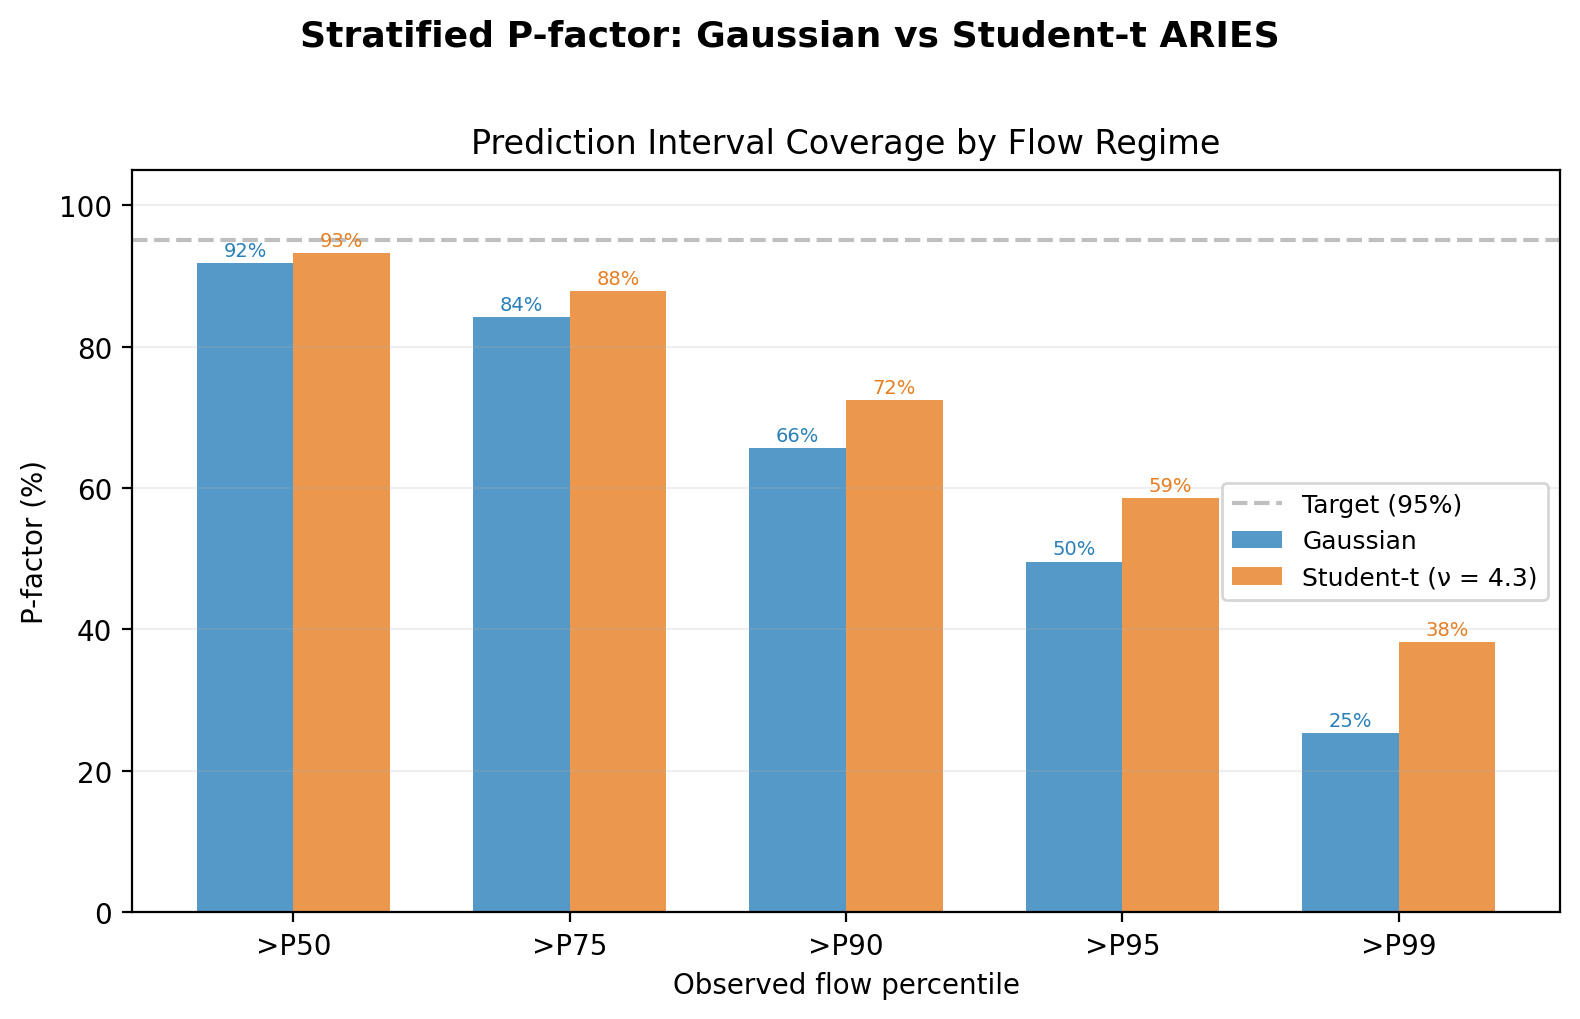
\includegraphics[width=0.85\textwidth]{figures/fig_student_t_stratified_pf.png}
\caption{Prediction interval coverage (P-factor) stratified by observed
         flow percentile.
         The Student-$t$ likelihood maintains higher coverage at all
         percentiles, with the largest improvement at extreme flows
         ($>\!P_{95}$, $>\!P_{99}$).
         Dashed line: nominal 95\% target.}
\label{fig:stratified}
\end{figure}

Figure~\ref{fig:ppc} shows the posterior predictive mean and 95\%
credible intervals for the first three years of the training period.
The Student-$t$ prediction intervals are visibly wider at the flood
peaks, capturing observations that fall outside the Gaussian intervals.
Near the mean flow, both likelihoods produce similar interval widths.

\begin{figure}[tbp]
\centering
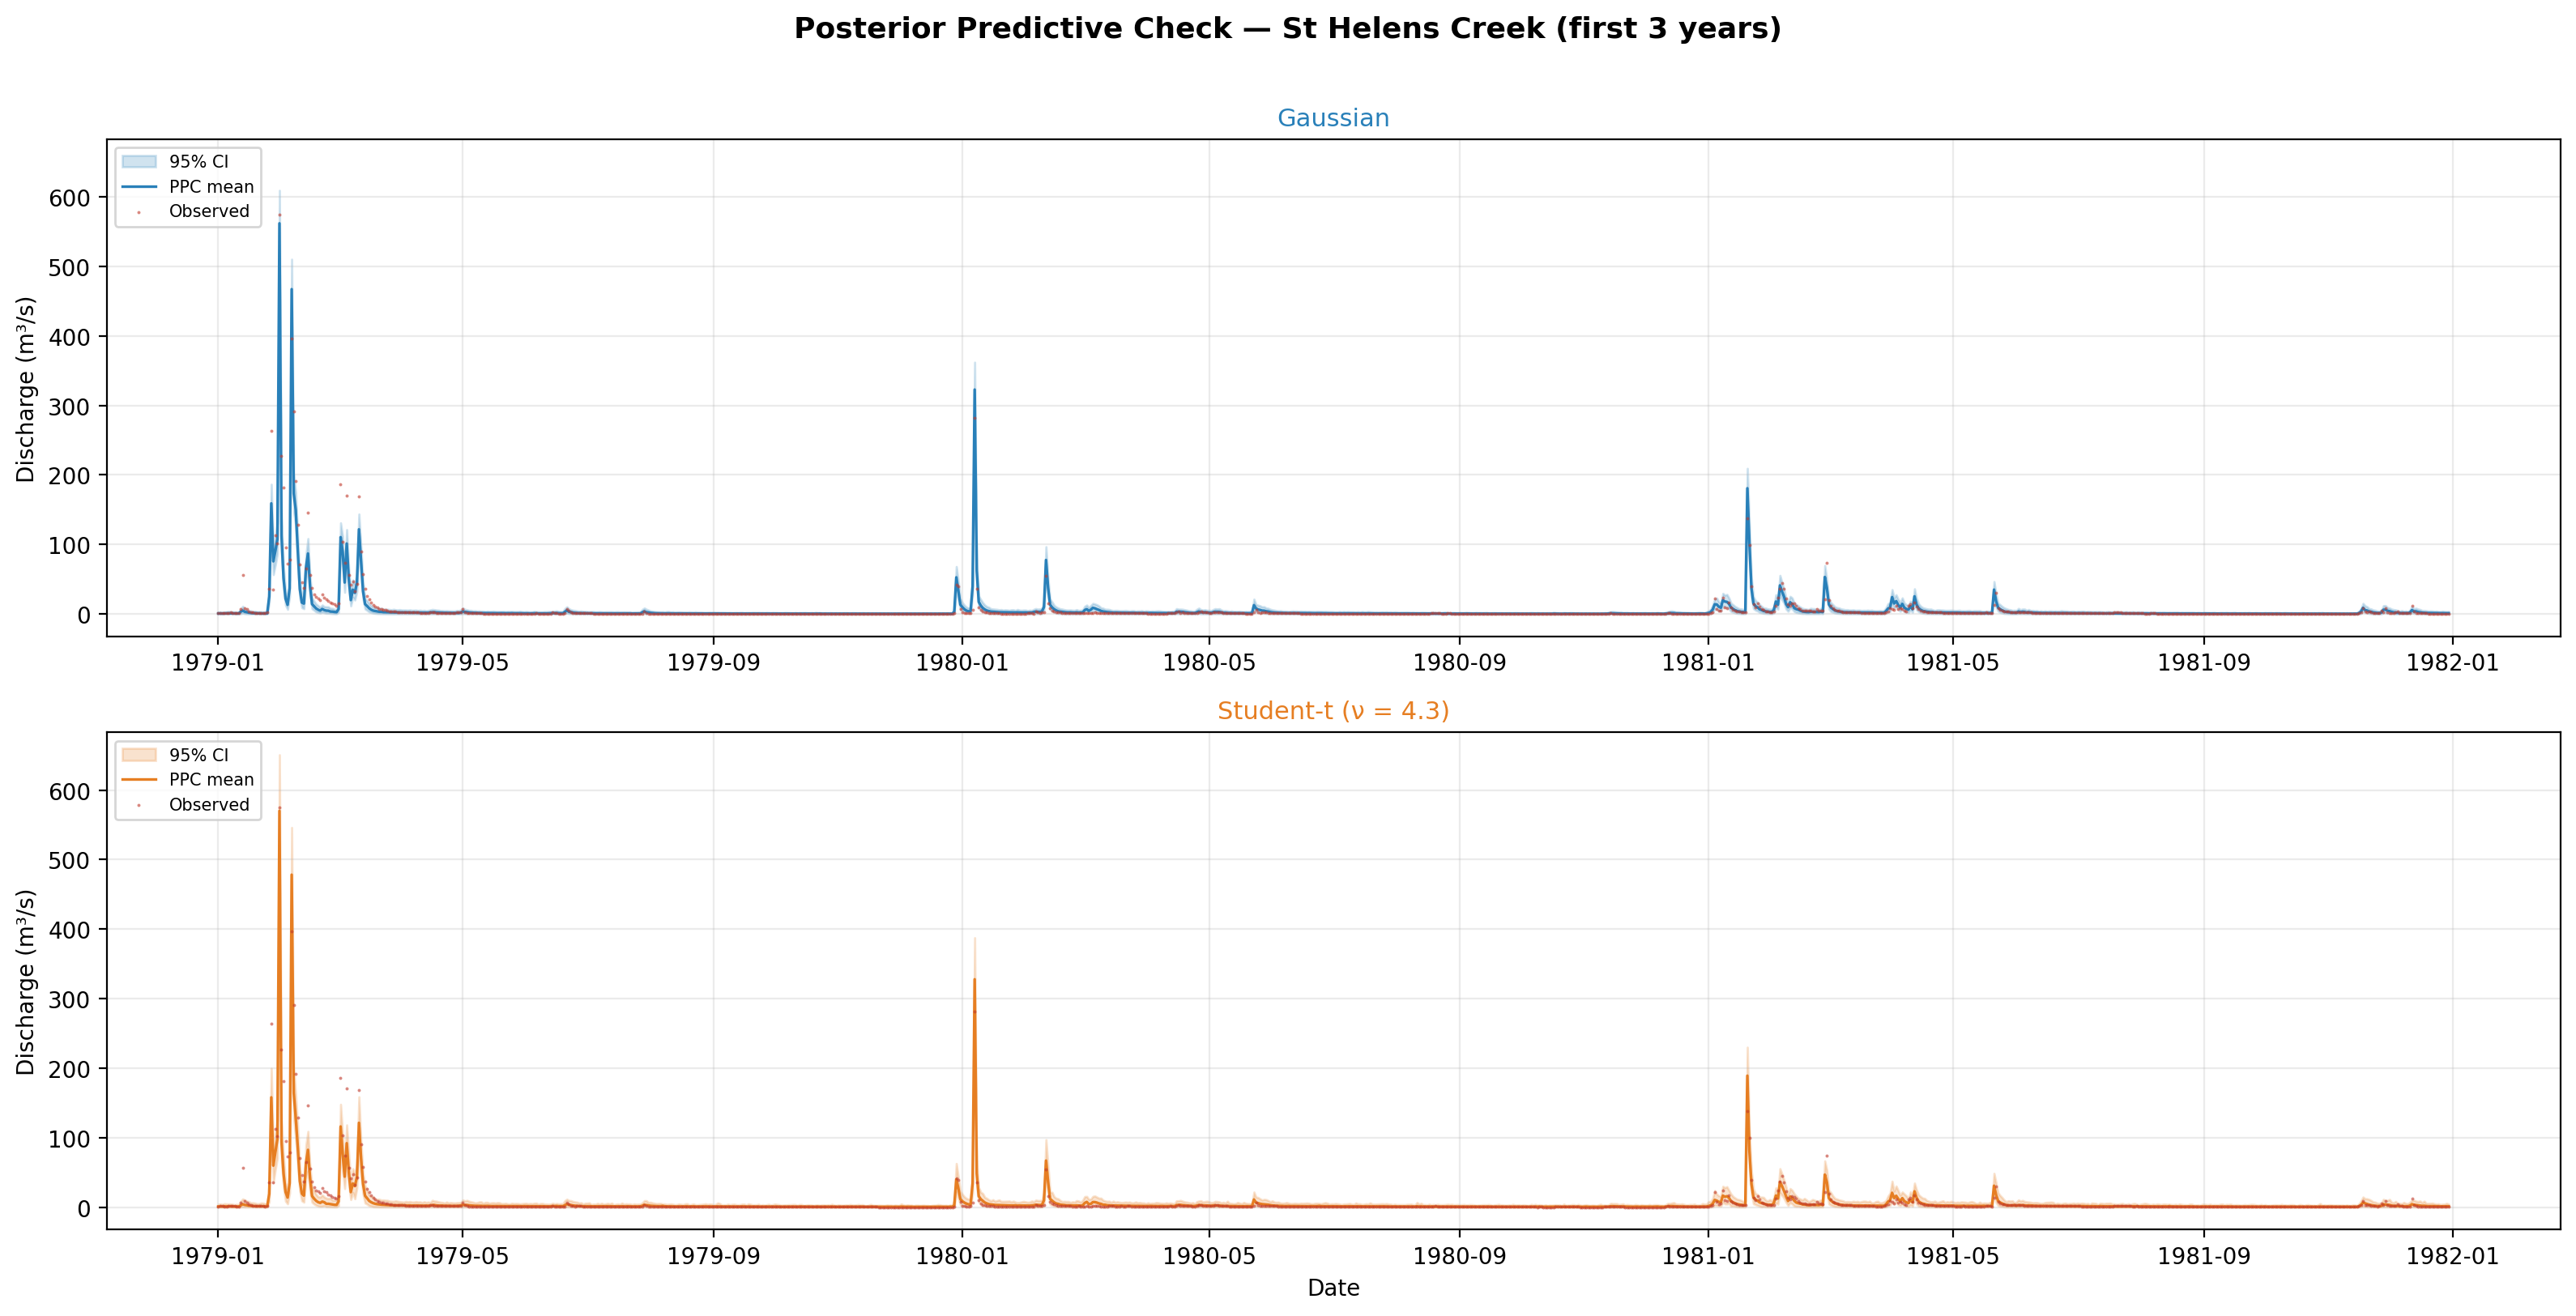
\includegraphics[width=\textwidth]{figures/fig_student_t_ppc.png}
\caption{Posterior predictive check for the first three years of the
         training period (1979--1981).
         Top: Gaussian likelihood.
         Bottom: Student-$t$ likelihood ($\nu = 4.3$).
         Orange band: 95\% credible interval.
         Orange line: posterior predictive mean.
         Red points: observed daily discharge.
         The Student-$t$ intervals are wider at flood peaks, capturing
         observations that fall outside the Gaussian intervals, while
         maintaining similar width near the mean flow.}
\label{fig:ppc}
\end{figure}

%=============================================================================
\section{Discussion}
%=============================================================================

\subsection{Why the Student-$t$ Works}

Three properties make the Student-$t$ likelihood particularly suitable
for ensemble Kalman methods.
First, the scale-mixture-of-normals representation~(\ref{eq:scale_mixture})
makes the implementation trivial---40 lines of code with no new inference
machinery.
Second, the separation of $\nu$ (tail heaviness) from $\phi$ (baseline
noise) means the adaptive noise estimation (IKEA) continues to operate
unchanged; $\phi$ estimates the typical observation error (with
$\lambda_i \approx 1$ for well-fit observations) while
$\lambda_i \ll 1$ selectively increases perturbation variance for
large residuals.
Third, $\nu$ is directly interpretable: $\nu = 4.3$ means the data
effectively contain occasional $10\sigma$--$20\sigma$ events that the
Gaussian model cannot accommodate without distorting $\phi$.

\subsection{Limitations}

The kurtosis-based $\nu$ estimator~(\ref{eq:nu_est}) assumes $\nu > 4$,
which is satisfied here but may not hold for datasets with extremely
heavy tails.
The EMA smoothing constant (0.7) was chosen heuristically; sensitivity to
this parameter has not been systematically explored.
The method does not address \emph{systematic} model structural error---
if the SAC-SMA model consistently underpredicts flood peaks (non-zero
mean residual at high flows), a heavier-tailed likelihood only partially
compensates.
A Kennedy--O'Hagan-style Gaussian process discrepancy
term~\cite{Kennedy2001} would be a natural extension for addressing
structured bias.

\subsection{Computational Cost}

The Student-$t$ extension adds negligible computational overhead.
Drawing $\lambda_i \sim \text{Gamma}$ for
$N_d = 11{,}323$ observations takes approximately 2~milliseconds.
The kurtosis computation requires one pass over the residuals.
Total per-iteration overhead is under 0.1~seconds on a standard desktop
workstation, compared to 8--12~seconds for the forward model evaluations
and Kalman update.
The full calibration (1,000 ensemble members $\times$ 12 iterations)
completed in approximately 120~seconds, identical to the Gaussian
baseline.

%=============================================================================
\section{Conclusion}
%=============================================================================

We have presented an adaptive Student-$t$ likelihood for the ARIES
ensemble smoother that provides robustness to outlier observations
without requiring changes to the Kalman update machinery.
The method adds approximately 40 lines of code, introduces no new
tuning parameters, and preserves the computational efficiency of the
Gaussian baseline.

Application to the St~Helens Creek catchment demonstrates that the
Student-$t$ likelihood improves probabilistic forecast calibration
(P-factor from 93.8\% to 96.2\% on validation data) while maintaining
identical point prediction accuracy (NSE = 0.87).
The adaptive $\nu$ converges to 4.3, confirming that daily discharge
residuals are substantially heavy-tailed.
Parameter estimates tighten consistently, with physically coherent
shifts from upper-zone fast-response storage toward lower-zone baseflow
storage.
The improvement in prediction interval coverage is concentrated at high
flows, where the consequences of forecast error are most severe.

The implementation is available as open-source software at
\url{https://github.com/frbennett/aries} and is integrated into the
main ARIES codebase.

\vspace{1em}
\noindent\textbf{Data and code availability:}
The complete workflow, including the self-contained Jupyter notebook,
model code, and forcing data, is available in the accompanying
repository.
SILO climate data are publicly available from the Queensland Government
Long Paddock website~\cite{Jeffrey2001}.
BOM Hydrologic Reference Station data are available from the Australian
Bureau of Meteorology~\cite{Zhang2014}.

%=============================================================================
\begin{thebibliography}{99}

\bibitem[Bennett(2026)]{Bennett2026}
  Bennett~F (2026).
  \newblock ``ARIES: Adaptive Residual-based Iterative Ensemble Smoother.''
  \newblock \emph{In preparation}.

\bibitem[Botha et al.(2023)]{Botha2023}
  Botha~I, Adams~MP, Tran~DH, Bennett~FR, Drovandi~CC (2023).
  \newblock ``Component-Wise Iterative Ensemble Kalman Inversion for
             Static Bayesian Models.''
  \newblock \emph{Statistics and Computing}, \textbf{33}, 109.

\bibitem[Burnash(1995)]{Burnash1995}
  Burnash~RJC (1995).
  \newblock ``The NWS River Forecast System---Catchment Modeling.''
  \newblock In Singh~VP (ed.), \emph{Computer Models of Watershed
             Hydrology}, pp.~311--366. Water Resources Publications.

\bibitem[Emerick and Reynolds(2013)]{Emerick2013}
  Emerick~AA, Reynolds~AC (2013).
  \newblock ``Ensemble Smoother with Multiple Data Assimilation.''
  \newblock \emph{Computers \& Geosciences}, \textbf{55}, 3--15.

\bibitem[Evensen(2003)]{Evensen2003}
  Evensen~G (2003).
  \newblock ``The Ensemble Kalman Filter: Theoretical Formulation and
             Practical Implementation.''
  \newblock \emph{Ocean Dynamics}, \textbf{53}, 343--367.

\bibitem[Gneiting and Raftery(2007)]{Gneiting2007}
  Gneiting~T, Raftery~AE (2007).
  \newblock ``Strictly Proper Scoring Rules, Prediction, and Estimation.''
  \newblock \emph{Journal of the American Statistical Association},
             \textbf{102}(477), 359--378.

\bibitem[Jeffrey et al.(2001)]{Jeffrey2001}
  Jeffrey~SJ, Carter~JO, Moodie~KB, Beswick~AR (2001).
  \newblock ``Using Spatial Interpolation to Construct a Comprehensive
             Archive of Australian Climate Data.''
  \newblock \emph{Environmental Modelling \& Software}, \textbf{16}(4),
             309--330.

\bibitem[Kennedy and O'Hagan(2001)]{Kennedy2001}
  Kennedy~MC, O'Hagan~A (2001).
  \newblock ``Bayesian Calibration of Computer Models.''
  \newblock \emph{Journal of the Royal Statistical Society: Series B},
             \textbf{63}(3), 425--464.

\bibitem[Lam et al.(2015)]{Lam2015}
  Lam~SK, Pitrou~A, Seibert~S (2015).
  \newblock ``Numba: A LLVM-Based Python JIT Compiler.''
  \newblock In \emph{Proceedings of the Second Workshop on the LLVM
             Compiler Infrastructure in HPC}, pp.~1--6.

\bibitem[Marshall et al.(2006)]{Marshall2006}
  Marshall~L, Sharma~A, Nott~D (2006).
  \newblock ``Modeling the Catchment via Mixtures: Issues of Model
             Specification and Validation.''
  \newblock \emph{Water Resources Research}, \textbf{42}, W11409.

\bibitem[Review(2025)]{Review2025}
  \newblock ``Beyond Normality: A Review of Heavy-Tailed Likelihoods for
             Robust Hydrological and Water Quality Prediction.''
  \newblock \emph{In press}.

\bibitem[Schoups and Vrugt(2010)]{Schoups2010}
  Schoups~G, Vrugt~JA (2010).
  \newblock ``A Formal Likelihood Function for Parameter and Predictive
             Inference of Hydrologic Models.''
  \newblock \emph{Water Resources Research}, \textbf{46}, W12515.

\bibitem[Smith et al.(2022)]{Smith2022}
  Smith~T, Marshall~L, McGlynn~B (2022).
  \newblock ``Diagnosing Hydrologic Model Structural Error Using
             Heavy-Tailed Likelihoods.''
  \newblock \emph{Water Resources Research}, \textbf{58}, e2021WR031376.

\bibitem[West(1987)]{West1987}
  West~M (1987).
  \newblock ``On Scale Mixtures of Normal Distributions.''
  \newblock \emph{Biometrika}, \textbf{74}(3), 646--648.

\bibitem[Zhang et al.(2014)]{Zhang2014}
  Zhang~SX, Bari~M, Amirthanathan~G, Kent~D, MacDonald~A, Shin~D (2014).
  \newblock ``Hydrologic Reference Stations to Monitor Climate-Driven
             Streamflow Variability and Trends.''
  \newblock In \emph{Hydrology and Water Resources Symposium 2014},
             pp.~1048--1055.

\end{thebibliography}

\end{document}
